% !TeX spellcheck = en_GB

\section{Experiments and Results}


\begin{figure}[t]
	\centering
	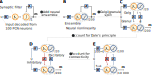
\includegraphics{media/chapter_cerebellum/network_types.pdf}
%	\begin{subfigure}{1.4in}%
%		\centering%
%		\includegraphics[scale=0.95]{media/network_types_a.pdf}%
%		\phantomcaption%
%		\label{fig:network_types_a}%
%	\end{subfigure}%
%	\begin{subfigure}{1.4in}%
%		\centering%
%		\includegraphics[scale=0.95]{media/network_types_b.pdf}%
%		\phantomcaption%
%		\label{fig:network_types_b}%
%	\end{subfigure}%
%	\begin{subfigure}{1.4in}%
%		\centering%
%		\includegraphics[scale=0.95]{media/network_types_c.pdf}%
%		\phantomcaption%
%		\label{fig:network_types_c}%
%	\end{subfigure}%
%	\begin{subfigure}{1.4in}%
%		\centering%
%		\includegraphics[scale=0.95]{media/network_types_d.pdf}%
%		\phantomcaption%
%		\label{fig:network_types_d}%
%	\end{subfigure}%
%	\begin{subfigure}{1.4in}%
%		\centering%
%		\includegraphics[scale=0.95]{media/network_types_e.pdf}%
%		\phantomcaption%
%		\label{fig:network_types_e}%
%	\end{subfigure}%
	\caption[Network types used in the cerebellum experiments.]{Network types used in our experiments. \textbf{(A)} \enquote{Direct} implementation with an optimal integrator. \textbf{(B)} Using the synaptic filter of a single population of spiking neurons for temporal integration. \textbf{(C)} Inter-neuron population in the recurrent path. \textbf{(D)} Same as \textbf{C}, but accounting for Dale's principle. \textbf{(E)} Same as \textbf{D}, but with more detailed biological constraints (see text).}
	\label{fig:network_types}
\end{figure}

\begin{figure}[t]
	\centering
	\includegraphics{media/chapter_cerebellum/2d_sweeps.pdf}
	\caption[Delayed signal reconstruction errors in the Cerebellum model.]{Delayed signal reconstruction error for different types of input signals, delays, and network types. All error values are expressed as RMSE divided by the average RMS of the input signal over ten trials. Columns correspond to the network types in Fig.~\ref{fig:network_types}. \emph{Top row:} Reconstruction error for rectangle pulse signals of varying width. \emph{Bottom row:} Reconstruction error for a band-limited white noise input signal with varying band-limit.}
	\label{fig:basic_results}
\end{figure}

\begin{figure}
	\centering
    \includegraphics{media/chapter_cerebellum/delay_example.pdf}
	\caption[Examples showing the delayed input signals decoded form the granule layer in the detailed model.]{Examples showing the delayed input signals decoded form the granule layer in the detailed model (Fig.~\ref{fig:network_types_e}). \emph{Top row:} Input signal (rectangle pulses in \textbf{A}, white noise in \textbf{B}). \emph{Middle row:} Spike raster for 40 randomly selected granule cells. \emph{Bottom row:} Delays decoded from one thousand randomly selected granule cells. Dotted lines correspond to an optimal delay.}
	\label{fig:sample_run}
\end{figure}

In the following, we discuss three experiments. First, we analyze the temporal representations produced by each of the increasingly constrained models described above. Second, we systematically vary model parameters to gain a better understanding of why certain parameters are as observed. Third, we extend our model to incorporate the remaining components of the cerebellar microcircuit discussed above, resulting in a complete model of eyeblink conditioning.

\subsection{Influence of biological constraints on temporal representations}

To evaluate the effects of these biological details, we systematically generate two different types of input $u(t)$, feed those into the network and record the resulting activity.
In particular, we present results with a periodic pulse input of varying pulse width $t_\mathrm{on}$ and band-limited white noise of varying bandwidth $B$. These are meant to depict typical sorts of inputs that may arise in experimental situations (pulses) and more real-world situations (band-limited white noise).
We then determine how accurately the past history of $u$ over the window $\theta$ can be recovered from the resulting network activity via optimal linear readout weights. We use $\theta = \SI{0.4}{\second}$ in all simulations; each individual experiment simulates the network for $T = \SI{10}{\second}$.
The error is the RMSE of the reconstruction divided by the RMS power of the input itself (normalized RMSE, or NRMSE).

The overall results for all five models are shown in Fig.~\ref{fig:basic_results}.
This shows the average reconstruction error for varying inputs (horizontal axis) and for varying time delays (vertical axis) over ten trials.
An example run of Model E (the model with the most biological detail) is shown in Fig.~\ref{fig:sample_run}.
The different decoded output lines (bottom) are all based on the same neural activity (middle), but with different readout weights.
These approximate the input value $u$ with various time delays over the entire time window, from the immediate input right now ($\theta'/\theta=0$) to $\theta$ seconds ago ($\theta'/\theta=1$).  

As can be seen in Fig.~\ref{fig:basic_results}, the network successfully functions as a method for encoding the temporal pattern of input data over the desired window of time $\theta$.
Adding more biological detail decreases the accuracy with which the system approximates \cref{eqn:delay_network_lti}, but most of the information is still encoded.
The pulse input (Fig.~\ref{fig:sample_run}A) shows that the reconstruction is a smoother version of the input; the system is not good at representing sudden changes, and this is the main source of noise in the reconstruction.  This is as expected from using smooth Legendre polynomials as temporal basis functions. Furthermore, we note that there is a peak in accuracy when decoding data from $\theta' = \SI{60}{\milli\second}$ in the past ($\theta'/\theta=0.15$), and this peak is more pronounced as more biological detail is added. This corresponds to the neurotransmitter time-constant $\tau = \SI{60}{\milli\second}$ we use for all connections, and which is based on a first-order low-pass fit to the NMDA Granule-Golgi dynamics reported in \citet{dieudonne1998submillisecond}. Note that the reported time-constants of other connections in the system are significantly shorter \cite{kanichay2008synaptic}. Techniques described by \cite{voelker2018improving} could be used to compute the connections weights for these heterogeneous time-constants. Yet, for the sake of simplicity, here we assume homogeneous time-constants.

\subsection{Parameter exploration}

\begin{figure}[t]%
%	\begin{subfigure}{0.26\textwidth}%
%		\centering%
%%		\includegraphics[trim=0.2cm 0.3cm 0.25cm 0.25cm,clip,scale=0.95]{media/sweep_tau.pdf}%
%		\phantomcaption%
%		\label{fig:sweep_tau}%
%	\end{subfigure}%
%	\begin{subfigure}{0.21\textwidth}%
%		\centering%
%%		\includegraphics[trim=0.25cm 0.3cm 0.25cm 0.16cm,clip,scale=0.95]{media/sweep_n_pcn_granule_convergence.pdf}%
%		\phantomcaption%
%		\label{fig:sweep_pcn_gr_conv}%
%	\end{subfigure}%
%	\begin{subfigure}{0.21\textwidth}%
%		\centering%
%%		\includegraphics[trim=0.25cm 0.3cm 0.25cm 0.125cm,clip,scale=0.95]{media/sweep_n_golgi_granule_convergence.pdf}%
%		\phantomcaption%
%		\label{fig:sweep_go_gr_conv}%
%	\end{subfigure}%
%	\begin{subfigure}{0.32\textwidth}%
%		\centering%
%%		\includegraphics[trim=0.25cm 0.3cm 0.25cm 0.1cm,clip,scale=0.95]{media/desired_vs_measured_pcn_convergence.pdf}
%		\phantomcaption%
%		\label{fig:convergence}%
%	\end{subfigure}
	\centering
	\includegraphics{media/chapter_cerebellum/parameter_sweeps.pdf}%
	\includegraphics{media/chapter_cerebellum/convergence_histogram.pdf}
	\caption[Cerebellum model parameter exploration.]{Parameter exploration. \textbf{(A-C)} Effects of varying parameters on the delay reconstruction error (arrows indicate default parameters). The box plots show the median, lower and upper quartile of all the data depicted as a contour plot in Fig.~\ref{fig:basic_results}; whiskers are the min/max. The total number of data-points in each bar plot is $n = 441$. \textbf{(D)} Histograms showing the frequency of measured PCN to granule convergences.}
	\label{fig:param_sweeps}
\end{figure}

Notably, we can use our model to determine what the accuracy would be like if we changed individual parameters, such as the aforementioned synaptic time-constant.
This is shown in Fig.~\ref{fig:sweep_tau}.
Interestingly, the performance of the system is best for a filter time-constant of \SI{50}{\milli\second}, which is closed to the value we used based on measured Granule-Golgi dynamics.

As discussed above, a striking feature of the cerebellar microcircuitry is the low granule cell convergence. One possible hypothesis is that these numbers are a trade-off between minimizing connectivity and the overall performance of the resulting system.
In our model, we can test this hypothesis by systematically varying the number of pre-neurons the solver has access to. Results are shown in Figs.~\ref{fig:param_sweeps}B and C.

For the PCN to Granule convergence (Fig.~\ref{fig:param_sweeps}B) the performance of the system does improve with larger limits, yet plateaus at still relatively small convergence numbers.
Importantly, as mentioned above, the specified desired convergence solely controls the number of \emph{potential} pre-neurons.
Since the neural weight solver may still set a weight to zero, these convergence numbers are strict upper limits.
Measuring the actual convergence in the PCN to granule connections (Fig.~\ref{fig:param_sweeps}D), we see a peak at one to three PC neurons connecting to each granule cell, and this peak is only weakly affected by the desired convergence number.
Importantly, in nature, PC neurons connect to on average four granule cells (see \cite{palkovits1972quantitative}, for the complete statistics), whereas we only measure an average convergence of two in our model (for a desired convergence of five).
We can match the observed average in our model by increasing the desired convergence to 13. This slightly increases the performance of the system and coincides with the optimal desired convergence depicted in Fig.~\ref{fig:param_sweeps}B.
Nevertheless, since the gain in performance is relatively small, we decided not to alter the desired convergence in our model setup.

Fig.~\ref{fig:param_sweeps}C indicates that the performance of the system improves up to a desired Golgi to granule convergence number of thirteen, with a measured average convergence of $4.8$ in the final network.
This is a little higher than what is commonly assumed in the neuroscience literature, although, notably, there is some uncertainty regarding this number.
The original study by \citet{jakab1988quantitative} on the physiology of individual glomeruli (the sites receiving Golgi cell axons and granule cell dendrites; cf.~Fig.~\ref{fig:cerebellum_anatomy}) counts up to 145 Golgi axon synapses in one glomerulus.
However, it is unclear whether these synapses originate from a single or different Golgi cells.
Most researchers assume at most one Golgi cell connecting to each glomerulus, and, as explained above, each granule cell in turn connecting to on average of four glomeruli \cite{palkovits1972quantitative}.
Our model predicts that if the Granule-Golgi circuit were to optimally generate a temporal basis, then multiple Golgi cells should sometimes connect to the same glomerulus.

\subsection{Extension Toward a Model of Eyeblink Conditioning}

Given the above model for the Golgi and granule cells, we can now introduce learning into the model to test the behavior of the system in an eyeblink conditioning task.
As discussed above, the error signal $\varepsilon(t)$ originates from the Inferior Olive (IO).
This signal needs to represent the difference between the conditioned response (CR; i.e., what the model has learned so far), and the unconditioned response (UR; i.e., the motor response produced by the innate eyeblink reflex).
These are the two inputs to the IO shown in \Cref{fig:cerebellum_anatomy}.
The CR is the inhibitory input from the Cerebellar Nucleus (CN), and the UR is the excitatory input from the PCN.  

To create a neural version of this, we use a similar approach as described in the second version of the Granule-Golgi circuit.
That is, we train a single-hidden-layer neural network for each of the IO, CN, and pRN using least-squares, and then combine the $\mat{D}$ and $\mat{E}$ matrices to form connection weights.
This is a standard technique when building NEF models.

To adjust the connection weights between the Granule cells and the Purkinje cells, we use the Prescribed Error Sensitivity (PES) rule defined by \citet{macneil2011finetuning}, a biologically plausible variant of the classic delta learning rule.
Let $w^{\mathrm{Gr}\to\mathrm{Pu}}_{ij}$ be the connection weight between the $j$th granule cell and the $i$th Purkinje cell, $\eta$ a learning rate parameter, $a^\mathrm{Gr}_j(t)$ the $j$th post-synaptic granule cell activity filtered by a low-pass filter with time-constant $\tau_\mathrm{learn}$, and $e^\mathrm{Pu}_i \in \{-1, 1\}$ the encoder of the $i$th Purkinje cell, determining whether this cell is an on- or off-neuron.
The delta learning rule is given as
\begin{align}
	\frac{d}{dt} w^{\mathrm{Gr}\to\mathrm{Pu}}_{ij}(t) &= -\eta \varepsilon(t) e^\mathrm{Pu}_i a^\mathrm{Gr}_j(t) \,.
	\label{eqn:delta}
\end{align}
This learning rule can be derived from gradient descent in a single-layer network.
For a small enough $\eta$, the weights are guaranteed to converge to the least-squares solution used in the previous experiments.
The PES rule is given by rewriting \cref{eqn:delta} in terms of local weights and activities
\begin{align*}
	\frac{d}{dt} w^{\mathrm{Gr}\to\mathrm{Pu}}_{ij}(t) &= -\eta \sum_{k} w^{\mathrm{IO}\to\mathrm{Pu}}_{ik} a^\mathrm{IO}_k(t) a^\mathrm{Gr}_j(t) \,,
\end{align*}
where $a^\mathrm{IO}_k(t)$ is the activity of the $k$th IO cell and $w^{\mathrm{IO}\to\mathrm{Pu}}_{ik}$ are the synaptic weights between the $k$th IO cell and the $i$th Purkinje cell. These weights are the product of the Purkinje cell encoder $e_i^\mathrm{Pu}$ and a decoding vector $\vec d_k^\mathrm{IO}$ that linearly decodes the error signal $\varepsilon(t)$ from IO cell activity.

\begin{figure}[t]
	\centering%
%	\includegraphics[]{media/results_panel.pdf}\\[-0.15cm]
	\caption[Model and experimental data for the eyeblink conditioning task.]{Model and experimental data for the eyeblink conditioning task. \textbf{(A, B)} Maximum CR triggered eyelid closure over 500 trials for six random instances of the model/experimental animals. Gray dots correspond to the eyelid closure at the time of the US. Black line is the moving average over 11 trials. Blue dotted lines correspond to an experimental day (100 trials). \textbf{(C, D)} Eyelid closure trajectory averaged over one experimental day and all six models/animals. \textbf{(E)} Eyelid velocity signal decoded at the Purkinje cells compared to the reflex-triggered velocity signal. Data for \textbf{(B, D)} adapted from \protect\citet{heiney2014cerebellardependent}.}
	\label{fig:result-basic}
\end{figure}

\Cref{fig:result-basic} shows the behaviour of a typical run of the detailed version of our model performing the eyeblink conditioning task over 500 trials.
The \enquote{tone} (CS) is modeled as a rectangle pulse with $t_\mathrm{on} = \SI{100}{\milli\second}$.
The \enquote{puff} (US) occurs \SI{250}{\milli\second} after the CS onset.
The model learns to have the eye closed when the puff occurs. Notably, individual instances of the network show slight differences in learning speed, just as individual experimental animals do.

While our model reproduces key features of eyeblink conditioning, its behavior differs from the experimental data in some aspects.
Foremost, the model does not reproduce the increase in learning speed over time; to the contrary, learning slows down as the model converges to the optimal set of parameters.
Furthermore, our model shows far less inter-trial variance compared to experimental animals.
We think that the reasons for this are twofold.
First, the $10\,000$ granule cells used in our experiments provide an on average very stable temporal basis from which we can decode the motor control signal.
Second, we do not model external systems that might interfere with the cerebellar motor commands, such as signals originating from motor cortex, or the physics of the eyelid itself.
Since these processes may be a significant source of inter-trial variance, it is not unsurprising that our model produces a relatively noise-free output.
Still, more research in these areas will be required in the future.

Most parameters were set based on biological data; the synaptic time-constant $\tau = \SI{5}{\milli\second}$ except in the Granule-Golgi microcircuit, as described above.
The only free parameters are the learning rate $\eta=140\times 10^{-6}$, $\tau_\mathrm{pRN} = \SI{100}{\milli\second}$ for the connections involving the pRN, and $\tau_\mathrm{learn} = \SI{60}{\milli\second}$ for filtering the granule cell activity in the learning rule.
The learning rate was adjusted to match the number of trials typically needed for mice to learn the task ($\sim 300$ trials).
Velocity commands smaller than $v_\mathrm{th} = \SI{2}{\milli\metre\per\second}$ are counted as zero.

The low-pass filter $\tau_\mathrm{learn}$ on the learning connection is required to reproduce the observation that the animal will close the eye slightly \emph{before} the puff occurs as learning progresses.
Without the additional filter the system learns to close the eye soon \emph{after} the puff.  This is because it is trying to do exactly what we have asked it to: learn to re-create the same motor pattern as is produced by the unconditioned reflex.  But, the unconditioned reflex closes the eye \emph{after} the puff happens, which is too late.  However, by slowing the passage of information from the Cerebellar Nucleus back to the Inferior Olive (where the comparison between the UR and CR occurs), we are effectively comparing the reflex at one point in time to the generated output from the cerebellum at an \emph{earlier} point in time.  This allows the new learned reflex to occur slightly earlier than the unconditioned response, and thus the eye closes before the air puff.  We note that this is a situation where adding biological detail (the synaptic filtering) improves the performance of the model.  If the model were to learn to \textit{exactly} reproduce the UR given the CS, then the eyeblink would occur \textit{after} the puff of air, which would be a less useful response.
